%%%%%%%%%%%%%%%%%%%%%%%%%%%%%%%%%%%%%%%%%
% Journal Article
% LaTeX Template
% Version 1.3 (9/9/13)
%
% This template has been downloaded from:
% http://www.LaTeXTemplates.com
%
% Original author:
% Frits Wenneker (http://www.howtotex.com)
%
% License:
% CC BY-NC-SA 3.0 (http://creativecommons.org/licenses/by-nc-sa/3.0/)
%
%%%%%%%%%%%%%%%%%%%%%%%%%%%%%%%%%%%%%%%%%

%----------------------------------------------------------------------------------------
%	PACKAGES AND OTHER DOCUMENT CONFIGURATIONS
%----------------------------------------------------------------------------------------

\documentclass[twoside]{article}

\usepackage{lipsum} % Package to generate dummy text throughout this template

\usepackage{graphicx}

\usepackage{placeins} % block floats

\usepackage{hyperref}
\makeatletter
\let\ref\@refstar
\makeatother

\usepackage{amsmath}

\usepackage[sc]{mathpazo} % Use the Palatino font
\usepackage[T1]{fontenc} % Use 8-bit encoding that has 256 glyphs
\linespread{1.05} % Line spacing - Palatino needs more space between lines
\usepackage{microtype} % Slightly tweak font spacing for aesthetics

\usepackage[hmarginratio=1:1,top=32mm,columnsep=20pt]{geometry} % Document margins
\usepackage{multicol} % Used for the two-column layout of the document
\usepackage[hang, small,labelfont=bf,up,textfont=it,up]{caption} % Custom captions under/above floats in tables or figures
\usepackage{booktabs} % Horizontal rules in tables
\usepackage{float} % Required for tables and figures in the multi-column environment - they need to be placed in specific locations with the [H] (e.g. \begin{table}[H])
%\usepackage{hyperref} % For hyperlinks in the PDF

\usepackage{lettrine} % The lettrine is the first enlarged letter at the beginning of the text
\usepackage{paralist} % Used for the compactitem environment which makes bullet points with less space between them

\usepackage{abstract} % Allows abstract customization
\renewcommand{\abstractnamefont}{\normalfont\bfseries} % Set the "Abstract" text to bold
\renewcommand{\abstracttextfont}{\normalfont\small\itshape} % Set the abstract itself to small italic text

\usepackage{titlesec} % Allows customization of titles
\renewcommand\thesection{\Roman{section}} % Roman numerals for the sections
\renewcommand\thesubsection{\Roman{subsection}} % Roman numerals for subsections
\titleformat{\section}[block]{\large\scshape\centering}{\thesection.}{1em}{} % Change the look of the section titles
\titleformat{\subsection}[block]{\large}{\thesubsection.}{1em}{} % Change the look of the section titles

\usepackage{fancyhdr} % Headers and footers
\pagestyle{fancy} % All pages have headers and footers
\fancyhead{} % Blank out the default header
\fancyfoot{} % Blank out the default footer
\fancyhead[C]{Augmented Novels $\bullet$ COS 401 - Srinivas Bangalore $\bullet$ Princeton University} % Custom header text
\fancyfoot[RO,LE]{\thepage} % Custom footer text



%----------------------------------------------------------------------------------------
%	TITLE SECTION
%----------------------------------------------------------------------------------------

\title{\vspace{-15mm}\fontsize{24pt}{10pt}\selectfont\textbf{Augmented Novels\thanks{This work is a final project for Srinivas Bangalore's class COS~401 in Princeton University}} } % Article title

\author{
\large
\textsc{Bill HUANG \& Gabriel HUANG}\\[2mm] % Your name
\normalsize Princeton University \\ % Your institution
\normalsize{billyanhuang@gmail.com\quad gabi.xiao.huang@gmail.com} % Your email address
\vspace{-5mm}
}
\date{}

%----------------------------------------------------------------------------------------

\begin{document}

\maketitle % Insert title

\thispagestyle{fancy} % All pages have headers and footers

%----------------------------------------------------------------------------------------
%	ABSTRACT
%----------------------------------------------------------------------------------------

\begin{abstract}

We design and implement a book reading aid, that we call Augmented Novels. Given any text, Augmented Novels
automatically identifies characters, extracts profiles, organizes text, and models relationships. We use a combination of natural language processing techniques including named entity recognition and knowledge bases such as WordNet. The resulting automatically-generated augmented novel, like conventional human-made aids, expedites and improves reading comprehension.

\smallskip
\noindent\textbf{Keywords.} book summarization, named-entity, natural language processing

\end{abstract}

%----------------------------------------------------------------------------------------
%	ARTICLE CONTENTS
%----------------------------------------------------------------------------------------

\begin{multicols}{2} % Two-column layout throughout the main article text

\section{Motivation}

\lettrine[nindent=0em,lines=3]{W}{}hich American student does not remember the beautiful pieces of literature they had to read in high-school? The Great Gatsby~\cite{fitzgerald1925great}, To Kill A MockingBird~\cite{lee2010kill}, The Grapes of Wrath~\cite{steinbeck2006grapes} are among the Top~10 favorites of literature teachers. They are indeed amazing exercises of style, and feature complex vocabulary and grammatical constructs. And yet an inexperienced reader could find their reading fastidious or even cumbersome. There are often more characters than one can retain on the first pass. Important information such as key events and shifts in character psychology can be buried in an ocean of descriptions, small talk, and stylistic effects. Finally, the length of the text might make it hard to contextualize a given scene or dialogue. We want to develop a tool to help readers understand novels, at least from a high-level perspective.

%------------------------------------------------

\section{Previous Work}

The straightforward approach to this problem is text summarization. Text summarization is a substantial sub-field of natural language processing, and numerous papers have been published (see for example~\cite{nenkova2012survey, gupta2010survey, das2007survey}). Approaches are typically supervised or unsupervised. 

Supervised methods require pairs of documents with manual summaries, which are used to train a classifier, such as a logistic regression, into characterizing sentences that make a good summary. Examples of such characteristics are the presence of named entities, the use of certain words/part-of-speech tags, and the location of the sentence in the document. 

Unsupervised methods generally require a corpus a documents. Each sentence from the document to summarize is weighted and thresholded. For instance words are assigned a \textsl{tf.idf} score~\cite{salton1988term}, and word scores are combined into sentence scores. Another approach views sentences as nodes in a graph with edge weights higher for semantically similar sentences. Then nodes with properties such as high connectivity or eigenvector centrality (e.g. high PageRank) get higher scores. Such an approach is implemented in the TextRank framework~\cite{mihalcea2004textrank} but defines the similarity between two sentences as their weighted intersection, which doesn't account for individual word semantics. We try to build on TextRank by using word vectors trained on the Google News dataset ~\cite{mikolov2013distributed}, and extending the word to word cosine distance to sentences. The results remain poor on book summarization tasks. One could think of using WordNet~\cite{miller1995wordnet} to incorporate better, hand-crafted semantics, but our general impression is that unlike news articles, most sentences in books only make sense in their context. Thus even sentences important to the story might actually only be loosely connected to surrounding sentences.

The approaches previously described, and in fact most of the literature focus on specific types of documents, namely: technical reports, papers, and news articles. The authors of ~\cite{mihalcea2007explorations} create a book summarization dataset and report poor F-scores after directly applying state-of-the-art methods to it. Instead they first segment the book into a dozen of \emph{segments} using normalized min-cuts~\cite{leighton1999multicommodity} on the graph which nodes are sentence-like text units (\emph{chunks}) and edge weights are cosine distances on modified \textsl{td.idf} vectors. Segments are themselves ranked using eigenvector centrality (e.g. PageRank) and used to rank the sentences. Finally the sentences with top scores generate the summary. The authors report F-scores around 0.41, while taking the first sentences of the book gives 0.33 against 0.53 for humans. From this approach we take the idea of hierarchically segmenting a book, but using simpler and more intuitive methods described in section~\ref{section:augmented}.

%------------------------------------------------

\section{Augmented Novels \label{section:augmented}}

Book summarization remains difficult: extractive summarization is still an open problem, let alone abstraction. There is no statistical guarantee on the result neither: even long summaries might throw away important information. Augmented Novels takes another approach by augmenting the original text with as much useful information as it can. The goals of our system are:
\begin{itemize}
\item \textbf{Annotating the original text}. The original text is segmented, annotated and important sentences are highlighted. Information is entirely preserved.
\item \textbf{Character Profiling}. Profiles and characteristics are extracted for each detected character.
\item \textbf{Character Interaction Analysis}. A graph is generated that summarizes the interactions between the characters. Characters in closer relationships will appear closer on the graph.
\end{itemize}


%------------------------------------------------

\section{Method \label{section:method}}

We implement the Augmented Novels concept entirely in Python with the help of NLTK~\cite{bird2009natural} and a few standard libraries. The Graph Visualization is generated using GraphViz's Neato engine~\cite{ellson2002graphviz}. The process typically takes less than 10 seconds to process a whole book.

\subsection{Text Segmentation}

We define text segments to be \emph{self-contained} and \emph{atomic} chunks of text. By self-contained we mean that there is enough text in the segment to describe an event, idea, state, without the rest of the book. By atomic we mean that no segment should be breakable into two valid segments.

In practice there is no simple way to account for the semantics of the text. Thus we approximate text segments by detecting paragraphs in the book and classifying them into \textbf{dialog segments} or \textbf{narration segments} based on punctuation heuristics. Dialog segments are merged together when they are separated by less than $k$ narration segments (typically $k=3$). This is actually a good approximation because of the way most writers organize their book. However, some paragraphs contain many semantic units, and others make only sense when taken together. We will experiment with the normalized min-cut approach of~\cite{mihalcea2007explorations} in the future.

\subsection{Character Detection}

Character detection is related to named-entity recognition. Typically a named-entity algorithm will return a list of detected entities and classify them in categories such as "PERSON", "PLACE", "DATE", "CURRENCY". The goal is then to cross-reference all mentions of the same character.

\paragraph{Named Entity Detection} The straightforward way is to part-of-speech tag the book, using NLTK, and then call the NLTK pre-trained named-entity detector. This has several drawbacks. Part-of-speech tagging of a whole book takes about 2 minutes, which makes it the bottleneck of the process. The error rate is still high, probably because named entities in books differ from the Penn TreeBank dataset~\cite{marcus1993building} the tagger was trained on. Moreover, the named-entity model marks nearly every entity as "PERSON". Capitalized common nouns are also marked as "PERSON". Most characters are discovered but false positives are very high.

Instead, we describe a two-pass learning/predicting approach which runs in a few seconds for a book and preserves recall with comparable precision.

\paragraph{Character Learning (First Pass)} In lieu of tagging, we select all groups of capitalized words not starting a sentence or containing titles ("Mr.", "Doctor", "Madame", ...). We accumulate all characters after removing titles. At this point there are a lot of false positives such as "Hot Springs", or "New York". We then use various sources of knowledge and rules to filter out non-characters, namely:
\begin{itemize}
\item WordNet~\cite{miller1995wordnet}, which we use to detect people versus objects
\item Lists of common first and last names
\item The 5000 most common english words (we could not find any exhaustive list of strict \emph{non} proper nouns)
\end{itemize}
The filtering rules, detailed in the source code, are conservative: they sacrifice precision for recall. We also threshold candidates occuring below a threshold.

We can now merge instances of the same character into what we call a \emph{character synset},  e.g. merge the instances "Harry", "Harry Potter", and "Mr. Potter" into the HARRY\_POTTER synset. The difficulty is to not merge instances sharing the same first or last name. Unique instances of the standard form
$$[Title]\quad First \quad Last$$
each defines a new synset. The non-standard-form instances are merged into the existing synsets. Finally the remaining instances define and merge into new synsets (e.g. someone always referred to by a first/last/nickname like "Voldemort"). 

\paragraph{Character Prediction (Second Pass)} We now have character synsets and instances in the text. We link each instance with the synset they share tokens with. When multiple synsets fit, we use \emph{recency}: the synset which occurred last is chosen. This is similar to the way humans solve the ambiguity, minus semantic context.

\paragraph{Coreference resolution} Often characters are referred to using pronouns (e.g. "he", "they", "I"). Coreference resolution is the task of determining which entity each pronoun refers to. We are interested in the case where these entities are the characters. Resolving coreferences helps us gain much more information on the characters, and the exact sentences where they appear. We will explore some techniques from~\cite{soon2001machine} in future work.


\subsection{Character Interaction Analysis}

Ideally, we want to detect social settings (or \textit{contingencies}) by answering: when do characters interact by having a conversation, physically interacting, or acknowledging each other's presence? A story can be seen as an accumulation of non-social and social settings. We approximate social settings as the conversations detected during text segmentation. We keep track of pairs of characters appearing in the same conversation, and use them to generate the interaction graph (see Figure~\ref{figure:gatsby_graph} for instance).

For now, pronouns are ignored. Characters taking part in conversations are not always mentioned (as in "..., said Nick"), and conversely they might talk of people not taking part in the conversation (e.g. "Who is that Gatsby?"). On the other hand, conversations are not the only social contingencies, and a semantic segmentation of the text might find more of them.


\subsection{Character Profiling}

Understanding characters is a difficult task for both humans and computers. In order to help readers more easily grasp the characters in a novel, we generate character profiles. Ideally, we would like to imitate character summaries as found in human-made aids. This, however, would be a daunting task, involving high-accuracy information extraction, reliable coreference resolution, some semantics, and automatic text generation. 
Instead, we opt to extract a few key words describing the characters: their personalities, their habits, their attitudes, etc.

For each word $w$ and character $c$ in the text, we assign the pair a relevance score based how often they appear close to one another:
\begin{align*}
r(w,c) &= \sum_{w_i} \sum_{c_j} \lfloor ae^{\left(-\frac{d(w_i, c_j)}{b}\right)^2}\rfloor
\end{align*}
Where $d(w_i, c_j)$ is the distance in word tokens between occurrences $w_i$ and $c_j$, and $a, b$ appropriate constants. 

We then perform a tf-idf analysis while considering the rarity of the word as well, as we want words that are associated with the character and carry significant meaning to have the highest scores:
\begin{align*}
s(w,c) &= \frac{r(w,c) - \log{p(w)}}{k + n_w}
\end{align*}
Where $p(w)$ is the number of times $w$ appears in the COCA corpus~\cite{wang2008good} and $k$ an appropriate constant. 

Finally for each character $c$ we return the set of words $w$ with highest scores $s(w,c)$, which make up the profile for that character.

\subsection{Text Highlighting}

We experiment with the $t\!f.id\!f.st\!f.is\!f$ sentence weighing scheme described in~\cite{mihalcea2007explorations}. We first segment the book into macroscopic semantic units (for instance into chapters), and choose the 20 newsgroups dataset from Scikit-Learn~\cite{pedregosa2011scikit} as our corpus. Then each word $w$ is scored by multiplying:
\begin{itemize}
\item $t\!f$ the number of occurrences of $w$ in the book
\item $id\!f$ the inverse of the number of documents in the corpus containing $w$
\item $st\!f$ the number of occurrences of $w$ in the current segment
\item $is\!f$ the inverse of the number of segments containing $w$
\end{itemize}
Finally scores for each sentence are added and longer sentences are penalized by the logarithm of their length.

%------------------------------------------------

\section{Results}

We applied Augmented Novels to \textit{The Great Gatsby}, an extract from \textit{Harry Potter and the Sorcerer's Stone}, \textit{To Kill a Mockingbird}, \textit{The Cont of Monte Christo}, and \textit{The Adventures of Sherlock Holmes}.

A screenshot of the reading interface is shown in Figure~\ref{figure:interface}.

The interactions graphs are shown in Figures~\ref{figure:gatsby_graph}~and~\ref{figure:harry_graph}. Stronger interactions are represented by thicker, opaque, and redder edges. Notice how for The Great Gatsby the model correctly captured the main characters and their closeness, but fail to merge Nick and Carraway (the narrator) because nobody calls him "Nick Carraway". False positives are also detected such as "Broadway", "June", or "England" but these appear in the name list we use. They could probably be disambiguated by parsing sentences where they appear. 

As for character profiles, here are the some of the detected word associations:

\vspace{1ex}

\underline{\smash{The Great Gatsby:}}

Mr. Tom Buchanan: \emph{listen, impatiently, said}

Dan Cody: \emph{yacht, anchor, jailor}

Catherine: \emph{sister, crazy}

\underline{\smash{To Kill a Mockingbird:}}

Miss Maudie Atkinson: \emph{street, across, sunhat}

Mr. Heck Tate: \emph{knife, sheriff, handed}

Mr. Bob Ewell: \emph{knife, fell, accused}

\underline{\smash{The Count of Monte Cristo:}}

Mr. Monte Cristo: \emph{island, count, lord}

Mlle. Merc\'edes: \emph{lovely, sacrifice, betrothed}

M. Beauchamp: \emph{journalist, editor, journal}

\vspace{1ex}

Though not always accurate, the generated word associations do generally provide information on the character. 

Finally, results for text highlighting on The Great Gatsby are given Figure~\ref{figure:highlight}. We observe that the highlighted sentences contain usually at least on character. We will evaluate the results using standard text summarization benchmarks in the future.

%------------------------------------------------

\section{Conclusion and Future Work}

In this paper we designed and implemented a book reading aid. We explored ideas from the text summarization literature, both for short documents and books, found their limits, and adapted them to aid reading. Our tool, Augmented Novels, helps reading by annotating the text and analyzing the characters. 

There are many possible immediate improvements to our system. Text segmentation can incorporate semantics using graph-cuts on a semantic graph made of sentences and their distances in meaning. Social contingency detection could be made more accurate by training a classifier into identifying them (features could be: punctuation, persence of certain words, occurrence of named entities). A hybrid approach for character detection could combine the speed of our current approach and filter out false positives by parsing the sentences where the potential false positives appear. We could also train a Random Forest~\cite{breiman2001random} to filter candidate characters based on their WordNet hypernyms. Pronoun resolution, nickname resolution, although hard problems on their own, would allow us to identify even more information on the characters. The social interaction graph can be made interactive: clicking the edge between two characters would return all their interactions. Plotting the social interaction graph at different times in the book could give insights on social dynamics.

In the long run, we would like to implement question answering. Example queries would be "Who is Sherlock Holmes's best friend?", "How does Harry Potter look like?", "Who is Tom Buchanan's mistress?". The machine would then answer by returning extracts of the book or even synthesizing an answer.

To conclude, we would like to thank our instructor Dr. Srinivas Bangalore for his advice and fruitful discussions.

The complete source code is available at \href{https://github.com/gabrielhuang/parse-novel}{https://github.com/gabrielhuang/parse-novel}


%----------------------------------------------------------------------------------------
%	REFERENCE LIST
%----------------------------------------------------------------------------------------
%\FloatBarrier
\bibliographystyle{apalike}
\bibliography{AugmentedNovels}

%----------------------------------------------------------------------------------------

\end{multicols}


\begin{figure*}
  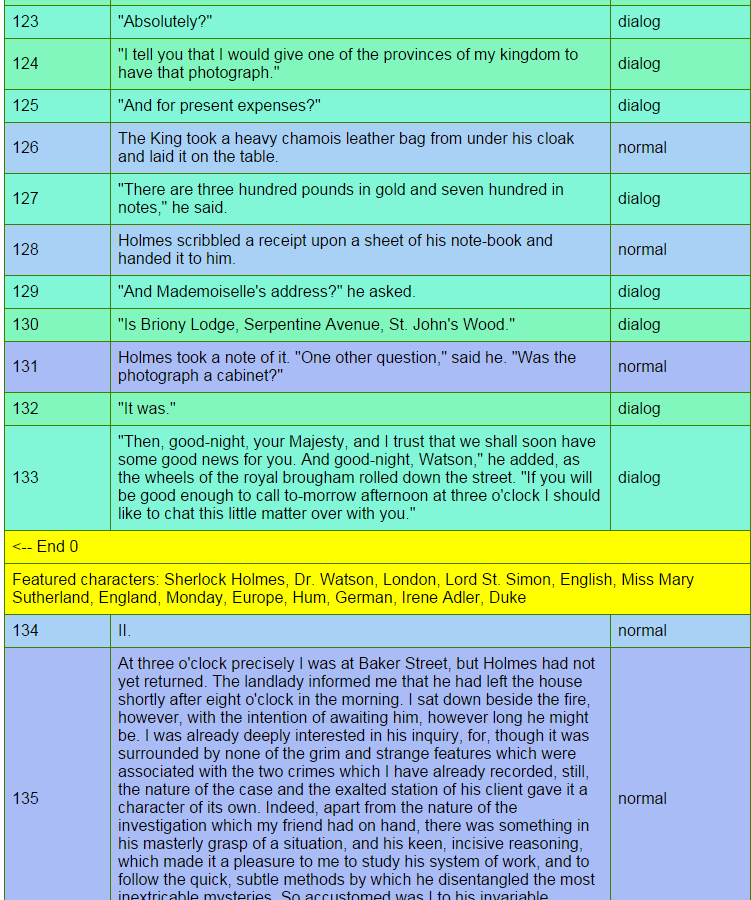
\includegraphics[width=\textwidth]{img/interface}
  \caption{Augmented Novels Reading Interface on \emph{The Adventures of Sherlock Holmes}\label{figure:interface}}
\end{figure*}

\begin{figure*}
  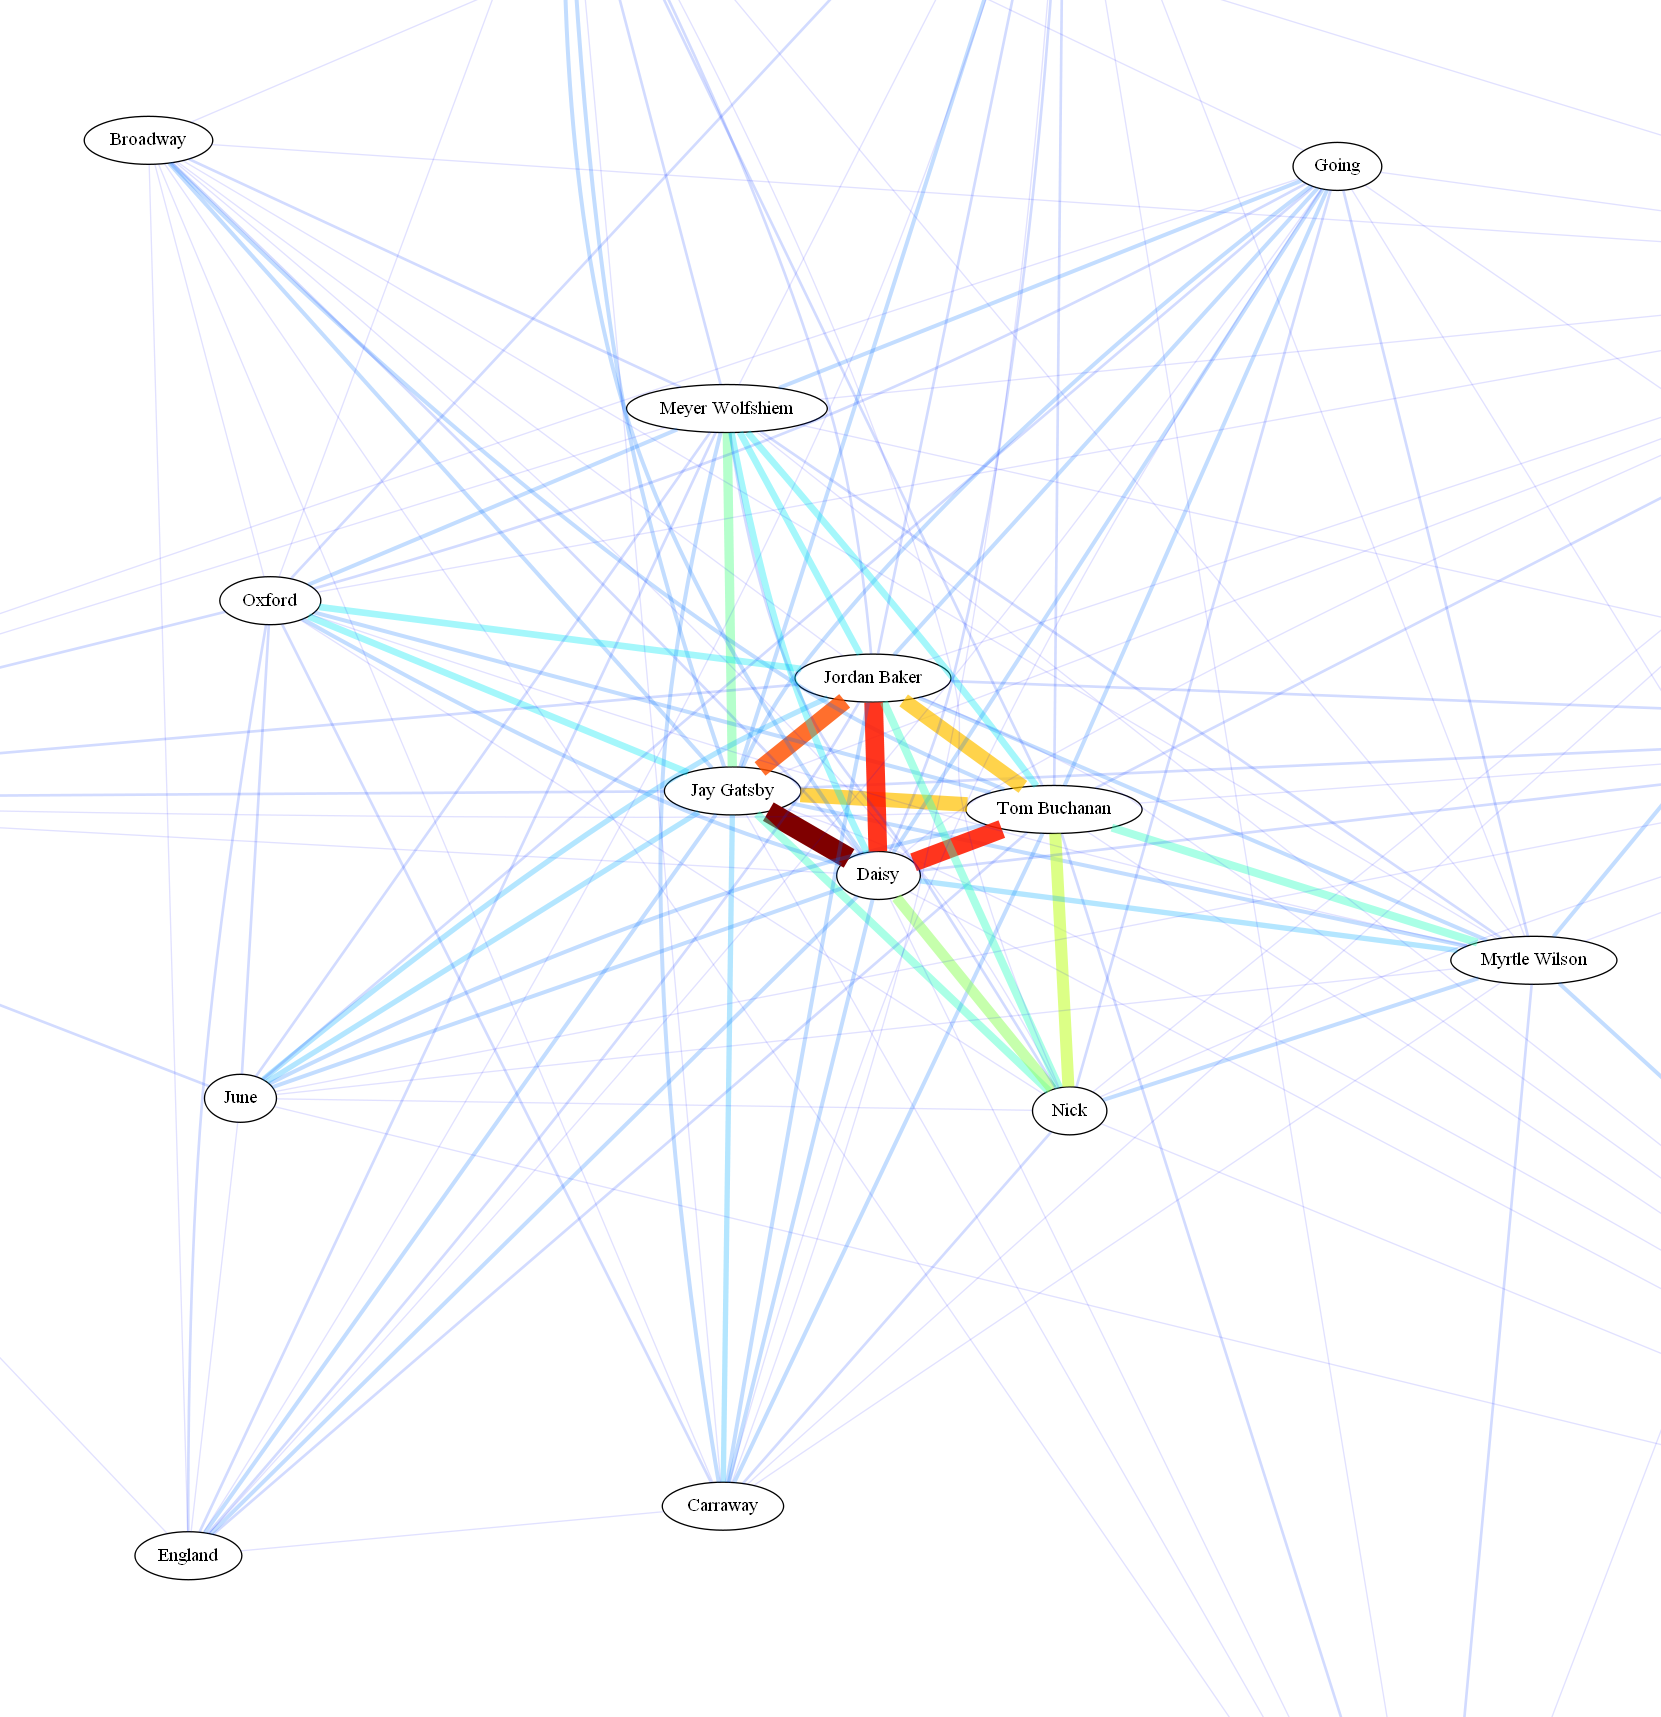
\includegraphics[width=\textwidth]{img/gatsby_full}
  \caption{Interactions of the Main Characters in \emph{The Great Gatsby}\label{figure:gatsby_graph}}
\end{figure*}

\begin{figure*}
  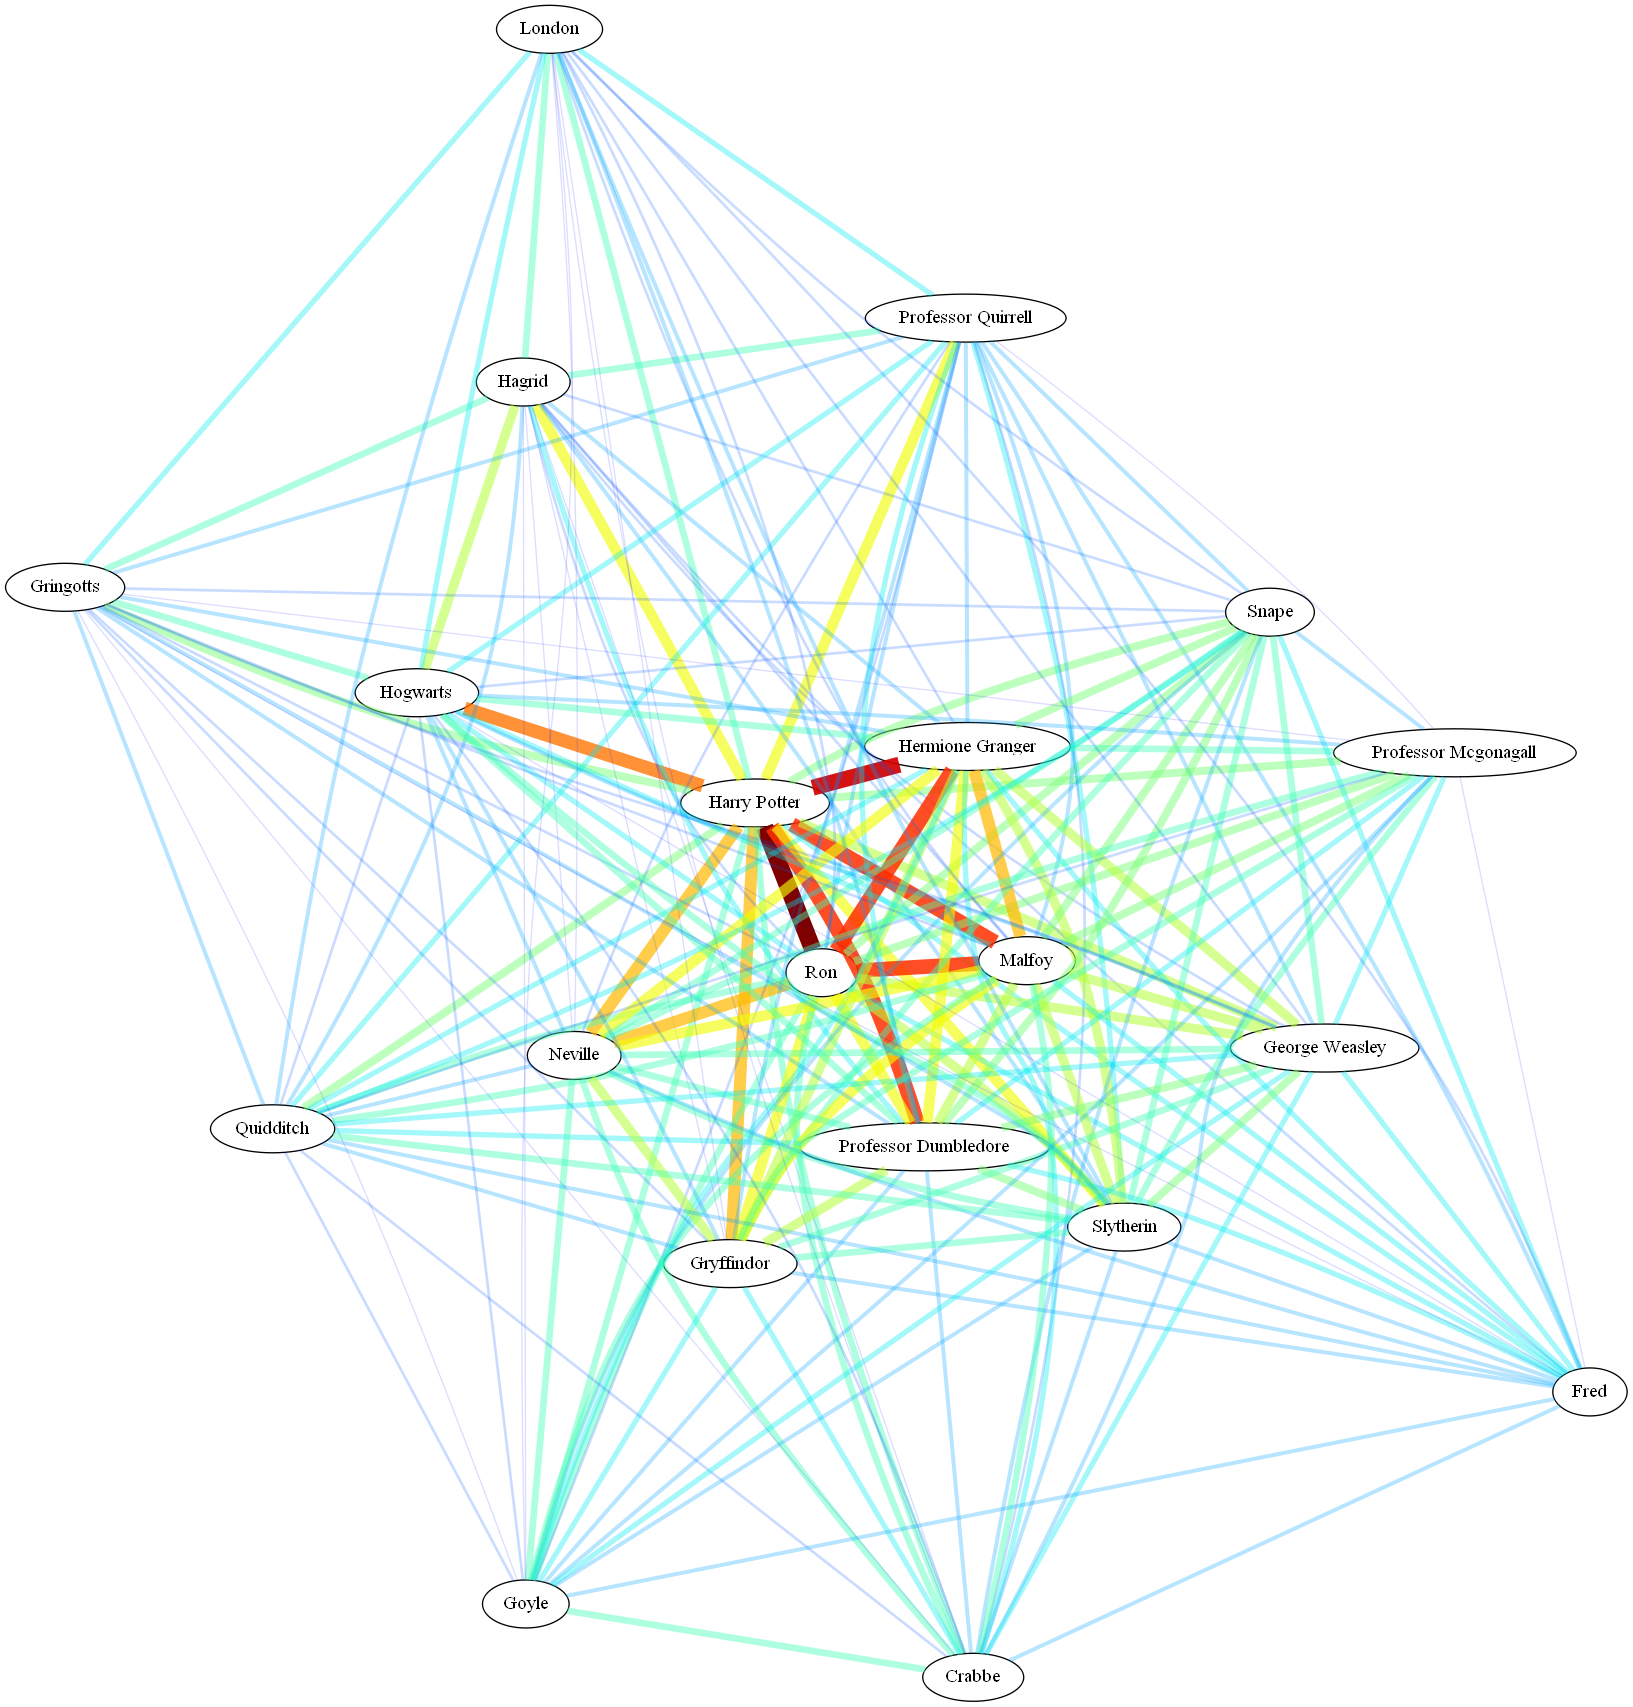
\includegraphics[width=\textwidth]{img/harry_full}
  \caption{Interactions of the Main Characters in \emph{Harry Potter and the Sorcerer's Stone}\label{figure:harry_graph}}
\end{figure*}

\begin{figure*}
\begin{center}
  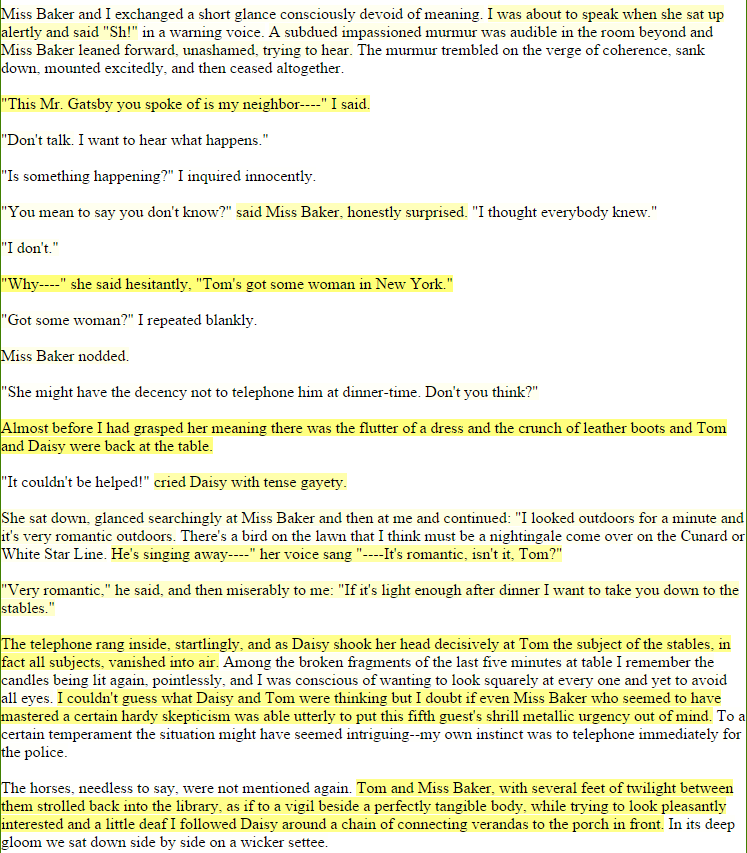
\includegraphics[width=0.8\textwidth]{img/highlight}
  \caption{Text Highlighting on \emph{The Great Gatsby}\label{figure:highlight}}
\end{center}
\end{figure*}

\end{document}